\chapter{Implementación}
     En este capítulo se explican los detalles de la implementación de las partes FrontEnd y BackEnd de nuestro proyecto, tanto de la generación del proyecto inicial como de la infraestructura del mismo.
    
    
    \section{FrontEnd}
    En esta sección se va a hablar del proyecto Angular el cual compone la parte FrontEnd de nuestra aplicación. Este framework nos ofrece un desarrollo más rápido con respecto a otros frameworks, ya que se estructura en diferentes componentes web y genera una página web dinámicamente.
    \subsection{Generación Proyecto Angular}
    Para la generación de un proyecto base en Angular se utilizó \textit{Angular Cli}, un herramienta de línea de comandos que facilita la creación y gestión de proyectos Angular y de sus diferentes componentes.
    \newline
    
    \textit{Angular Cli}, al tratarse de  una herramienta NodeJS, requiere tenerlo instalado en nuestro sistema operativo. Para ello la primera tarea a realizar es instalar NodeJS a través de su página oficial\cite{nodejs}, escogiendo la versión que soporte nuestro sistema operativo.
 
    A continuación, a través del terminal que nos proporciona la herramienta de desarrollo \textit{Visual Studio Code}, ejecutamos el comando \texttt{npm install -g @angular/cli@latest}, el cual nos instala \textit{Angular Cli} en la última versión disponible.
    
    \begin{figure}[h]
    \centering
     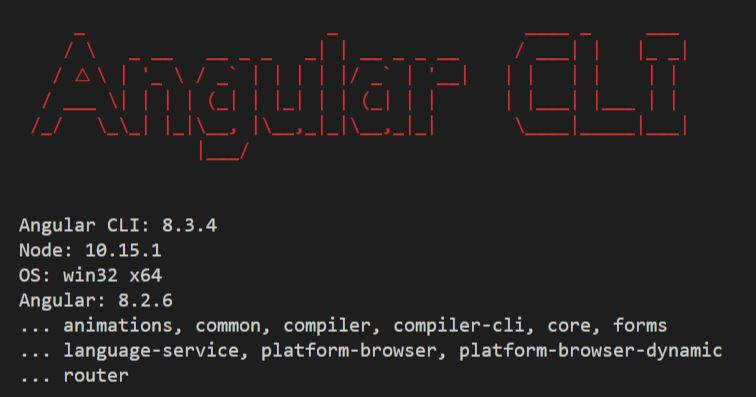
\includegraphics[width=0.65\textwidth]{images/angularversion}
    \caption{Versión Angular Cli}
    \end{figure}
    
    \FloatBarrier
    
    Una vez instalada la herramienta de comandos \textit{Angular Cli}, procedemos a crear nuestro proyecto base Angular ejecutando el comando \texttt{ng new estudio-medico-tfg2019}, generando un proyecto completo Angular junto con toda su estructura de carpetas.
    
    
    
    \subsection{Arquitectura de la aplicación Angular}
    
    \subsection{Inicialización del proyecto}
        \subsubsection{\underline{Local}}
        \subsubsection{\underline{Remoto}}
    
    
    \section{BackEnd}
    
     En esta sección se va a hablar del proyecto Java Spring Boot el cual compone la parte BackEnd de nuestra aplicación. La aplicación es una API-REST, la cual será consumida por el FrontEnd mediente llamadas en protocolo HTTP. 
     
     
    \subsection{Generación Proyecto Java Spring Boot}
    Para la generación del proyecto inicial se utilizó Spring Initializr\cite{springinitializr}, a través de su página web. Escogimos gestionar las dependencias del proyecto con Maven dado el alto grado de familiaridad que poseemos con esta tecnología. A continuación se escogió el lenguaje Java para implementar la aplicación debido a sus características intrínsecas(polimorfismo y herencia). Para finalizar se añadieron los paquetes de Web y JPA, necesarios para gestionar las conexiones externas y para la capa de persistencia.
    
    \begin{figure}[h]
    \centering
     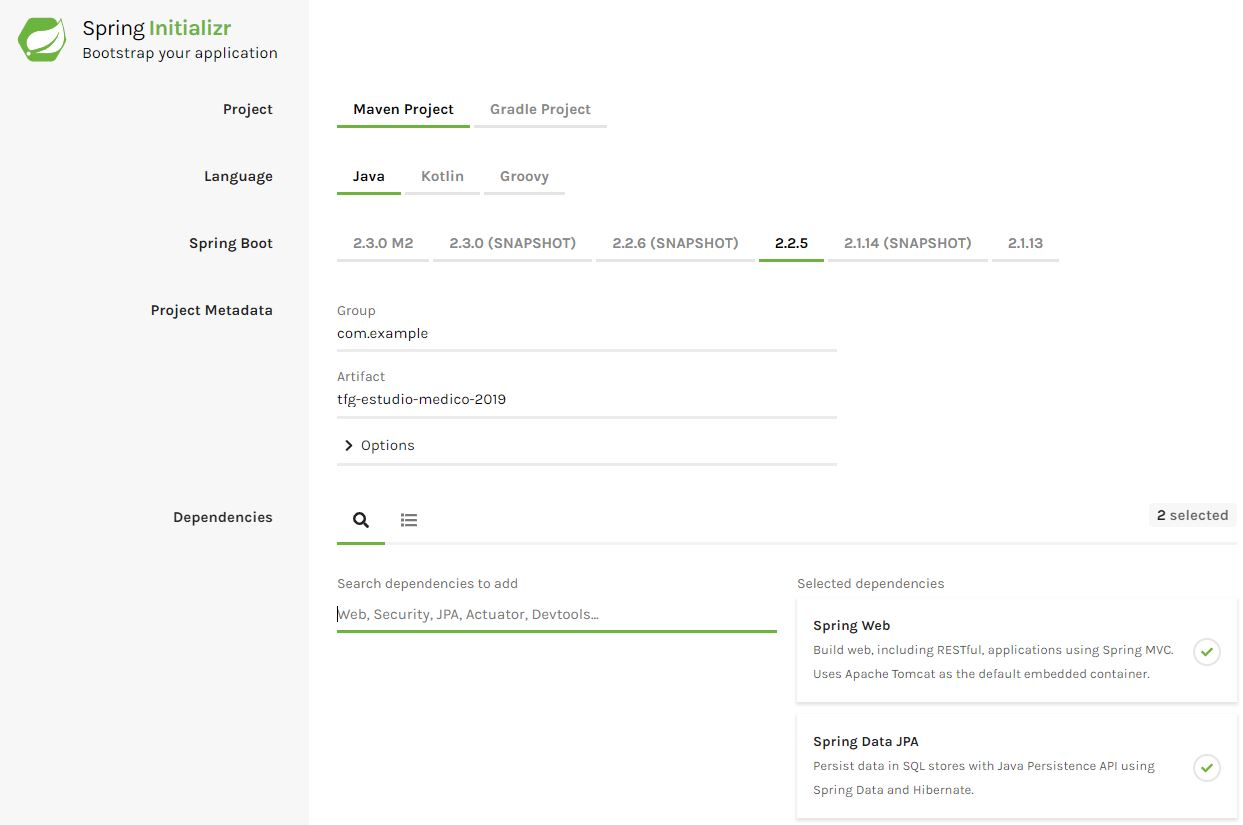
\includegraphics[width=1\textwidth]{images/springstarter}
    \caption{Proyecto inicial Spring Boot}
    \end{figure}
    
    Una vez generado el proyecto Sprinig Boot, hubo de importarse el mismo en el entorno de desarrollo Eclipse.
    
    
    \subsection{Arquitectura de la aplicación Java Spring Boot}
    La aplicación Spring Boot desarrollada se divide principalmente en los apartados de código, documentación y calidad

        \subsubsection{\underline{Código}}
        El proyecto BackEnd de la aplicación está escrito en Java 8, y dividido en los sigueintes bloques o paquetes, los cuales se describen a continuación.
        
        \begin{itemize}
            \item\textbf{Controladores}  \\
            Son los elementos del código encargados de recibir las diferentes peticiones HTTP y mapear los objetos enviados en las mismas, ya sea en el cuerpo de la petición en caso de ser una petición de tipo POST, o en la propia url si es una petición de tipo GET. Además de esto, son los encargados de realizar la lógica de navegación, llamando a la capa de negocio y, con el resultado obtenido, generar una respuesta a la parte FrontEnd de la aplicación.
            \newline
            
            Para identificar los diferentes controladores de nuestra aplicación, la nomenclatura de los mismos siempre terminará con la palabra \textit{Controller}.
            \newline
            
            En nuestra aplicación disponemos de 3 controladores: El \textit{UserController}, encargado principalmente del proceso de login de la aplicación. El \textit{AdminController}, encargado de obtener todos los recursos que demande el usuario de tipo administrador en nuestra aplicación. Finalmente el \textit{ResearcherController}, encargado de obtener los recursos que demanden los usuarios de tipo investigador en nuestra aplicación.
            \newline
            
            Todos los controladores se han implementado con el patrón de Diseño \textit{Interface}, separando los métodos de su implementación y haciendo al código más legible y mantenible de cara al futuro.
            \newline
            
                \begin{figure}[h]
                    \centering
                     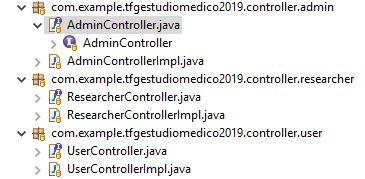
\includegraphics[width=0.8\textwidth]{images/controllers.JPG}
                    \caption{Controladores del proyecto BackEnd}
                \end{figure}
                
                \begin{figure}[h]
                \centering
                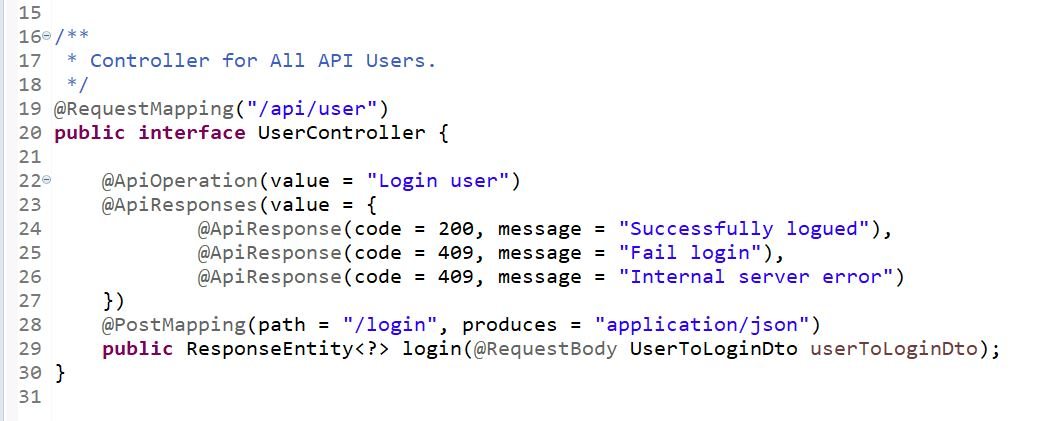
\includegraphics[width=1\textwidth]{images/usercontroller.JPG}
                \caption{Interfaz Controlador UserController}
                \end{figure}
                
                \FloatBarrier
            
             \item\textbf{Servicios de la aplicación}  \\
            Son los elementos del código encargados de centralizar la lógica principal de la aplicación. Los controladores los llaman, estos llaman a los repositorios para obtener los recursos solicitados, y devuelven dichos recursos al controlador.
            \newline
            
            Para identificar los diferentes servicios de de nuestra aplicación, la nomenclatura de los mismos siempre terminará con la palabra \textit{Business}.
            \newline
            
            En nuestra aplicación disponemos de 3 servicios de aplicación: El \textit{UserBusiness}, encargado principalmente de gestionar a los diferentes usuarios de la aplicación. El \textit{ResearcherBusiness}, encargado de gestionar las diferentes funcionalidades que puede realizar un usuario de tipo investigador en nuestra aplicación. Por último el \textit{SubjectBusiness}, encargado de gestionar a los pacientes y a sus respectivas citas y cuestionarios.
            \newline
            
             \begin{figure}[h]
                \centering
                
\includegraphics[width=0.8\textwidth]{images/business.JPG}
                \caption{Servicios de Aplicación del proyecto BackEnd}
            \end{figure}
            
            \begin{figure}[h]
                \centering
                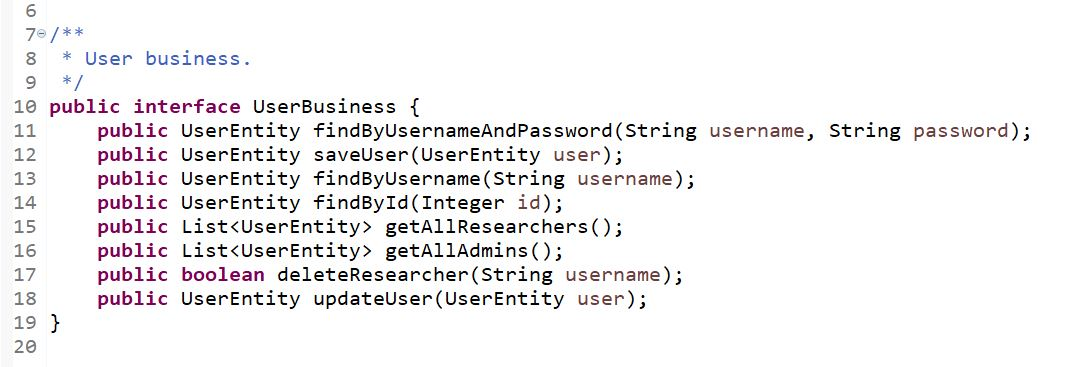
\includegraphics[width=1\textwidth]{images/userbusiness.JPG}
                \caption{Interfaz Servicio de aplicación UserBusiness}
            \end{figure}
            
            \FloatBarrier
            
            \item\textbf{Repositorios}  \\
            Son los elementos encargados de comunicarse con la base de datos correspodiente, ya sea guardando recursos, actualizar, listar, borrar etc... \\
            \newline
            Todos los repositorios extienden de la clase \textit{JpaRepository}, una clase perteneciente a SpringData, la cual implementa el código necesario para realizar una query a la base de datos. De esta manera no ha sido necesario implementar dichas clases.
            \newline 
            
            Para identificar los diferentes repositorios de de nuestra aplicación, la nomenclatura de los mismos siempre terminará con la palabra \textit{Repository}.
            \newline
            
            Nuestra aplicación dispone de 4 repositorios: El \textit{InvestigationDetailsRepository}, encargado de gestionar los detalles de los cuestionarios realizados a los pacientes. El \textit{InvestigationRepository}, encargado de gestionar los cuestionarios realizados a los pacientes. El \textit{UserRepository}, encargado de gestionar a los diferentes usuarios administradores e investigadores de la aplicación. Y finalmente, el
            \textit{SubjectRepository}, encargado de gestionar a los pacientes del estudio.
            \newline
            
            \begin{figure}[h]
                \centering
                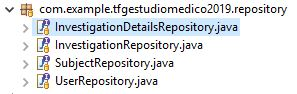
\includegraphics[width=0.8\textwidth]{images/repository.JPG}
                \caption{Repositorios del proyecto BackEnd}
            \end{figure}
            
            \begin{figure}[h]
                \centering
                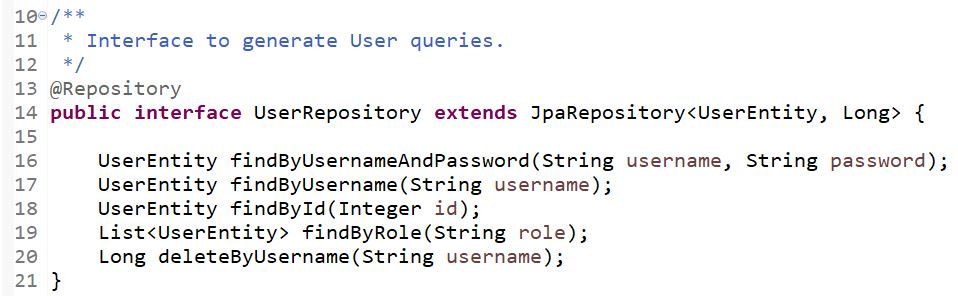
\includegraphics[width=1\textwidth]{images/userrepository.JPG}
                \caption{Interfaz Repositorio UserRepository}
            \end{figure}
            
            \FloatBarrier
            
            \item\textbf{Modelos}  \\
        \end{itemize}
        \subsubsection{\underline{Documentación}}
        \subsubsection{\underline{Calidad}}

        
        
    \subsection{Inicialización del proyecto}
        \subsubsection{\underline{Local}}
        \subsubsection{\underline{Remoto}}
    